%\documentclass[a4paper]{article}
\documentclass[times]{nlaauth}%
\usepackage{graphicx}

\usepackage{booktabs}
\usepackage{amsmath}
\usepackage{amsfonts}
\usepackage{amssymb}

% definitions used by included articles, reproduced here for 
% educational benefit, and to minimize alterations needed to be made
% in developing this sample file.

\newcommand{\pe}{\psi}
\def\d{\delta} 
\def\ds{\displaystyle} 
\def\e{{\epsilon}} 
\def\eb{\bar{\eta}}  
\def\enorm#1{\|#1\|_2} 
\def\Fp{F^\prime}  
\def\fishpack{{FISHPACK}} 
\def\fortran{{FORTRAN}} 
\def\gmres{{GMRES}} 
\def\gmresm{{\rm GMRES($m$)}} 
\def\Kc{{\cal K}} 
\def\norm#1{\|#1\|} 
\def\wb{{\bar w}} 
\def\zb{{\bar z}} 


\def\div{{\rm div}}
\def\Laplace{\Delta}
\def\grad{\nabla}
\def\supp{{\rm supp}}
\def\dist{{\rm dist}}
%\def\chset{\mathbbm{1}}
\def\chset{1}

\def\Tr{{\rm Tr}}
\def\sgn{{\rm sgn}}
\def\to{\rightarrow}
\def\weakto{\rightharpoonup}
\def\imbed{\hookrightarrow}
\def\cimbed{\subset\subset}
\def\range{{\mathcal R}}
\def\leprox{\lesssim}
\def\argdot{{\hspace{0.18em}\cdot\hspace{0.18em}}}
\def\Distr{{\mathcal D}}
\def\calK{{\mathcal K}}
\def\FromTo{|\rightarrow}
\def\convol{\star}
\def\impl{\Rightarrow}
%\DeclareMathOperator*{\esslim}{esslim}
%\DeclareMathOperator*{\esssup}{ess\,sup}
%\DeclareMathOperator{\ess}{ess}
%\DeclareMathOperator{\osc}{osc}
%\DeclareMathOperator{\curl}{curl}

%\def\Ess{{\rm ess}}
%\def\Exp{{\rm exp}}
%\def\Implies{\Longrightarrow}
%\def\Equiv{\Longleftrightarrow}
% ****************************************** GENERAL MATH NOTATION
\def\Real{{\rm\bf R}}
\def\Rd{{{\rm\bf R}^{\rm 3}}}
\def\RN{{{\rm\bf R}^N}}
\def\D{{\mathbb D}}
\def\Nnum{{\mathbb N}}
\def\Measures{{\mathcal M}}
\def\d{\,{\rm d}}               % differential
\def\sdodt{\genfrac{}{}{}{1}{\rm d}{{\rm d}t}}
\def\dodt{\genfrac{}{}{}{}{\rm d}{{\rm d}t}}

\def\vc#1{\mathbf{\boldsymbol{#1}}}     % vector
\def\tn#1{{\mathbb{#1}}}    % tensor
\def\abs#1{\lvert#1\rvert}
\def\Abs#1{\bigl\lvert#1\bigr\rvert}
\def\bigabs#1{\bigl\lvert#1\bigr\rvert}
\def\Bigabs#1{\Big\lvert#1\Big\rvert}
\def\ABS#1{\left\lvert#1\right\rvert}
\def\norm#1{\bigl\Vert#1\bigr\Vert} %norm
\def\close#1{\overline{#1}}
\def\inter#1{#1^\circ}
\def\ol#1{\overline{#1}}
\def\ul#1{\underline{#1}}
\def\eqdef{\mathrel{\mathop:}=}     % defining equivalence
\def\where{\,|\,}                    % "where" separator in set's defs
\def\timeD#1{\dot{\overline{{#1}}}}

% ******************************************* USEFULL MACROS
\def\prtl{\partial}                                        % partial deriv.
\def\Names#1{{\scshape #1}}

% ******************************************* DOCUMENT NOTATIONS
% document specific
\def\rh{\varrho}
\def\th{\vartheta}
\def\dx{\,\d\vx}
\def\dt{\,\d t}
\def\eps{\varepsilon}
\def\phi{\varphi}

\def\todo#1{\textcolor{red}{TODO: #1} }

%EndMSIPreambleData
%\providecommand{\U}[1]{\protect\rule{.1in}{.1in}}
\newtheorem{theorem}{Theorem}
%\newtheorem{algorithm}[theorem]{Algorithm}
%\newtheorem{assumption}[theorem]{Assumption}
%\newtheorem{axiom}[theorem]{Axiom}
\newtheorem{corollary}[theorem]{Corollary}
\newtheorem{definition}[theorem]{Definition}
\newtheorem{lemma}[theorem]{Lemma}
\newtheorem{notation}[theorem]{Notation}
\newtheorem{remark}[theorem]{Remark}
%\newcommand{\codename}[1]{\textsl{#1}}

%***************************************************************************
\begin{document}
 

\title
{Discrete Couplings for Mixed-Hybrid Formulation of Fracture Flow on Non-matching Grids of Different Dimensions}
\author{
Jan~B{\v r}ezina\affil{1} and
Pavel Burda\affil{2}
}
\runningheads{J. B\v rezina, P. Burda}
{Discrete Couplings for MHFEM on Non-matching Grids}
\address{
\affilnum{1}
Faculty of Mechatronics, Informatics and Interdisciplinary Studies,
Technical University of Liberec,
H\'alkova~6,~461~17~Liberec~1, Czech Republic
\break\affilnum{2}
TBD
}
%\cgs{
%This work was supported by the Technology Agency of the Czech Republic under the project no. TA01021331. }
%}
%\corraddr{J. {\v S}{\'\i}stek,
%Institute of Mathematics,
%Academy of Sciences of the Czech Republic,
%\v Zitn\' a~25, 115~67~Prague~1, Czech Republic.
%E-mail: sistek@math.cas.cz}
%
\begin{abstract}
\todo{abstrakt az casem}
\end{abstract}
%
\keywords
{non-matching grids, mixed-hybrid methods, analytical solution, fractured porous media, subsurface flow}%
%
\maketitle


\section{Introduction}
Realistic modeling of subsurface water flow has to deal with highly heterogeneous and multi-scale nature of the
hydraulic properties of the rock masses. The water moves slowly on the majority of the rock volume through
microscopic pores and fractures while it moves rapidly on the small part of the rock volume occupied by larger fractures
that forms preferential flow paths. These paths may by highly localized and the volumetric flow 
rate in them may be comparable or even dominating flow rate in the bulk volume. However, 
a cross-section of the larger fractures is still 
very small compared to the length scale of the whole domain, thus one has to refine computational mesh along the fractures 
in order to render them properly, 
which can lead to the meshes that are intractably larger, especially if  the network of fractures is dense enough. 
To overcome these difficulties, we consider the flow on fractures to be constant in the normal direction
and we integrate the flow equations over the aperture of the fractures. Similar procedure can be done for the channels
 with relatively
small cross-section area. Finally, we obtain system of equations on the domains of different dimension, coupled through the boundary 
conditions. This approach has been proposed by several authors, see e.g. \cite{reichenberger_mixed-dimensional_2006} or
homogenization arguments in \cite{martin_modeling_2005}.  

Even after this simplification, it could be difficult to obtain the mesh where the elements on the fractures match the sides of 
the elements of a surrounding continuum. The aim of this paper is to present two mortar-like methods for mixed-hybrid formulation
that relax this compatibility condition. Since these methods can not capture the jump in the pressure over the fractures, we have
to assume continuous pressure in our model. This is not completely unrealistic, since such a model can be viewed 
as a dual continuum model
in spirit of Gerke and Genuchten \cite{GerkeGenuchten1993a} where the fracture zone is explicitly localized. 

The paper is organized as follows. In the next section, we specify our model. Then, in Section 3,  we introduce its mixed-hybrid formulation.
The two new methods for discretization on incompatible meshes are presented in Section 4 and the last section is devoted to 
the numerical test of convergence of the methods.


\section{Problem formulation}
Let $\Omega_3$ be a domain in $\Real^3$, $\Omega_2\subset \Real^3$
a domain of fractures formed by piecewise smooth manifolds, and $\Omega_1 \subset \Real^3$ 
a domain of channels formed by piecewise smooth curves.
In order to keep further formulas consistent, we also introduce  $\Omega_0$ as the set of 
channel intersections. We assume that $\Omega_1$ has no direct interaction with $\Omega_3$, i.e.
\begin{equation}
  \Omega_{1}\cap\Omega_3 \subset \Omega_2.
\end{equation}
We also assume that the boundary of $\Omega_{d}$ is outside of $\Omega_{d+1}$ for $d=1,2$.
On the other hand, the domain $\Omega_d$ can hang out of $\Omega_{d+1}$ for $d=1,2$.

On these domains, we consider the Darcy's law 
\begin{equation}
 \label{darcy_equation}
 \vc{q}_d = \nu_d \vc v_d = -\nu_d \tn{K}_d \grad h_d   \quad\text{on }\Omega_d \setminus\Omega_{d-1}\quad \text{for }d=1,2,3;
\end{equation}
and the continuity equation
\begin{equation}
   \label{continuity_equation}
   \div \vc{q}_d = F_d                          \quad \text{on }\Omega_d\setminus\Omega_{d-1} \quad \text{for }d=1,2,3;
\end{equation}
where  $\vc v_d$ $[ms^{-1}]$ is the velocity $\vc{q}_d$ is the Darcy flux and $\nu_d$ is the measure of cross-section. 
The physical units of these quantities depends on the dimension
\begin{align*}
    &\vc{q}_3\ [ms^{-1}], &&\nu_3\  [-] &&\text{is constantly one,} \\
    &\vc{q}_2\ [m^2s^{-1}], &&\nu_2\ [m] &&\text{is fracture's aperture,}\\
    &\vc{q}_1\ [m^3s^{-1}], &&\nu_1\ [m^2] &&\text{is channel's cross-section area.}
\end{align*}
Other quantities in \eqref{darcy_equation} and \eqref{continuity_equation} are: the tensor of hydraulic conductivity $\tn{K}_d$,
the pressure head $h_d$ $[m]$, and  partially integrated density of the water sources $F_d$.
Vectors $\vc{q}_d$ and tensors $\tn{K}_d$ lives in the corresponding local tangent spaces of domains $\Omega_d$. The principal unknowns of this system 
are the fluxes $\vc{q}_d$ and the pressure heads $h_d$.

To complete the system, we have to prescribe boundary conditions. The boundary of $\Omega_d\setminus\Omega_{d-1}$ 
consists of the outer boundary $\prtl\Omega_d$ and
the interior interface to the domain $\Omega_{d-1}$. On the outer boundary, we consider the Dirichlet boundary condition $h_d=H_d$ 
on the set $\Gamma_d^D$ and the homogeneous Neumann 
boundary condition on the set $\Gamma_d^N$, where these two sets forms disjoint decomposition of $\prtl\Omega_d$. 
The boundary conditions on the interior interfaces introduce a coupling between dimensions. 
For $d=3$, the set $\Omega_2\cap\Omega_3 \setminus \Omega_1$ consists of separated patches of smooth two side manifolds,
 thus we need two boundary conditions on them.
First condition is the continuity of $h_3$ on both sides of the patch and the second is balance of the fluxes
\begin{equation}
  \label{eq:flux32}             
  \vc{q}_3^+ \cdot \vc n^+ + \vc{q}_3^- \cdot \vc n^- = Q_{3} = \sigma_{2}(\Tr\, h_3 - h_2).
\end{equation}
Here $Q_3$ is the surface density of the local outer flux from $\Omega_3$ into $\Omega_2$ which is proportional to the difference between
the trace of $h_3$ and $h_2$ with a given transition coefficient $\sigma_2$ $[s^{-1}]$. The flux $Q_3$ also appears as a part of 
the volume source $F_2 = Q_{3} +\nu_2 f_2$ on the domain $\Omega_2$. For $d=2$, the set $\Omega_1\cap\Omega_2 \setminus \Omega_0$ 
consists of separated curve segments, where every segment is  
on the boundary of $k\ge2$ different 2d-patches. The continuity of the pressure $h_2$ yields $k-1$ conditions 
and the last condition is again balance of the fluxes
\begin{equation}
  \label{eq:flux21}
  \sum_{i=1}^{k} \vc{q}_2^i \cdot \vc n^i = Q_{2} = \sigma_{1}(\Tr\, h_2 - h_1).
\end{equation}
Here $\sigma_1=\nu_2 \tilde\sigma_1$, where $\tilde\sigma_1$ $[s^{-1}]$ is the transition coefficient,  and
as before the flux $Q_{2}$ is a part of the volume source on $\Omega_1$, i.e. $F_1 = Q_{2} +\nu_1 f_1$. 
Similarly, we assume continuity of the pressure head $h_1$ and zero flux balance on the set $\Omega_0$ 
and for the consistency, we introduce $Q_1=0$.
Finally, we set $F_3=f_3$, where $f_d$ $[s^{-1}]$ is the density of external volume sources. For the sake of simplicity, we consider
equations \eqref{eq:flux32} and \eqref{eq:flux21} also on hanging parts, namely on $\Omega_2\setminus\Omega_1$ and $\Omega_1\setminus\Omega_0$ respectively,
but we set $\sigma_{d}=0$ on $\Omega_d\setminus\Omega_{d+1}$ for $d=1,2$.


\section{Mixed-Hybrid Formulation}
\todo{ Chceme opravdu nediskretni MH formulaci? Pokud ano, rozsirit zaver o existinci a jednoznacnosti}

\label{mathematical_formulation}
After introduction of the model, we are going to derive its mixed-hybrid weak formulation in the similar fashion as in 
\cite{brezina_mixed-hybrid_2010} and  \cite{maryska_mixed-hybrid_1995}.
To avoid technicalities, we assume that $\Omega_3$ have piecewise polygonal boundary, domain $\Omega_2$ consists of polygons, and
$\Omega_1$ consists of line segments. We also assume that the Dirichlet boundary $\Gamma_3^D$ 
is a polygonal subset of $\prtl\Omega_3$. 
Further, we decompose $\Omega_d$, $d=1,2,3$, into sub-domains $\Omega_d^i$, $i\in \mathcal{I}_d$,
and we denote the set of their boundaries
\[
 \Gamma_{d}=\bigcup_{i\in \mathcal{I}_d} \prtl\Omega_d^i.
\]
For now, we consider only the decompositions satisfying the compatibility condition
\begin{equation}
 \Omega_{d-1}\cap\Omega_{d} \subset \Gamma_d,\quad d=1,2,3,
 \label{eq:compatible}
\end{equation}
but we shall relax this condition on the discrete level.

In the following, we introduce spaces for the solution and the test functions. The fluxes $\vc q_d^i$ on the sub-domains 
$\Omega_d^i$ shall be from
\begin{equation}
    \label{Vspace}
        V=V_3\times V_2\times V_1=
                \prod_{d=3,2,1} \prod_{i\in \mathcal{I}_d} H(\div,\Omega_d^i),
\end{equation}
where $H(\div,\Omega_d^i)\subset L^2(\Omega_d^i)^d$ is the standard space of vector functions with divergence in 
$L^2(\Omega_d^i)$. The pressure head $h_d$ shall be from the space
\begin{equation}
        P_d=L^2(\Omega_d),
\end{equation}
and the trace of the pressure head $\mathring h_d$ from the space
\begin{equation}
        \mathring{P}_d=
           \Big\{\mathring{\phi}\in H^{\frac12}(\Gamma_d)\where \mathring{\phi}=0 \text{ on } \Gamma_d^D\Big\},
\end{equation}
where $H^{\frac12}(\prtl\Omega)$ is the space of traces of functions from $H^1(\Omega)$. Equivalently, it can be introduced
as the subspace of functions form $L^2(\Omega)$ with a finite norm
\begin{equation}
 \label{eq:frac_H_norm}
 \norm{u}_{H^\frac12(\Omega)}^2 = \int_\Omega u^2(x)\d x + \int_\Omega\int_\Omega \frac{\abs{u(x)-u(y)}^2}{\abs{x-y}^{d+1}}\d x \d y.
\end{equation}
In particular, $\mathring{P}_1$ is just finite-dimensional vector space. 
We also introduce common space for the pressure head unknowns
\begin{equation}
            P=P_3\times P_2\times P_1\times 
          \mathring{P}_3\times \mathring{P}_2\times \mathring{P}_1.
\end{equation}

In order to derive the mixed-hybrid formulation, we divide  \eqref{darcy_equation} by $\nu_d\tn K_d$, 
multiply it by a vector test function $\vc \psi_d \in V_d$,
and integrate by parts over every sub-domain~$\Omega_d^i$.
There appears a boundary term containing the trace of the pressure head $\mathring{h}_d$ which is further treated as an independent unknown. 
It can also be viewed as the Lagrange multiplier for the balance constrain
\begin{equation}
 \label{balance_constrain}
 \sum_{i\in \mathcal{I}_d} \vc q_d\cdot \vc n |_{\prtl\Omega_d^i} = \left\{ 
    \begin{array}{ll}
      Q_{d}\quad  &\text{on } \Omega_{d-1}\cap \Gamma_d,\\
      0    \quad  &\text{on } \Gamma_d \setminus \Omega_{d-1}, 
    \end{array}
 \right.
\end{equation}
imposed on the fluxes by \eqref{eq:flux32}, \eqref{eq:flux21} and their continuity out of $\Omega_{d-1}$.
Next, we substitute for $F_d$  in the continuity equation \eqref{continuity_equation}
and test it by $-\phi_d \in P_d$. Finally, we  substitute for $Q_d$ in the balance constrain \eqref{balance_constrain} 
and test this equation by the functions $\mathring\phi_d \in \mathring P_d$
with support on $\Gamma_d \setminus \Gamma_d^D$. After these manipulations, we arrive at 
following definition of the mixed-hybrid solution in terms of an abstract saddle point problem:
\begin{definition}
\label{MH-sol}
We say that pair $(\vc{q}, \ol{h})=\big(\vc{q},(h,\mathring{h})\big)\in V\times P$ is mixed-hybrid solution of the problem $P_{123}$
if it satisfies abstract saddle point problem
\begin{align}
        \label{Saddle1}
    a(\vc{q},\vc \psi) + b(\vc\psi, \ol{h}) 
    &= \langle G, \vc \psi\rangle &&\forall\, \vc\psi\in V,\\
        \label{Saddle2}
 b(\vc{q}, \ol\phi) - c(\ol{h},\ol\phi) &= \langle F, \ol\phi \rangle &&\forall\, \ol\phi=(\phi, \mathring{\phi}) \in P,
\end{align}
where the bilinear forms on the left-hand side are
\begin{align*}
 a(\vc q, \vc \psi)&=\sum_{d=1,2,3}\sum_{i\in \mathcal{I}_d} \int_{\Omega_d^i}
   \frac{1}{\nu_d} \vc q_d^i \tn K_d^{-1} \vc \psi_d^i,\\
%
 b(\vc q, \ol\phi)&=\sum_{d=1,2,3}\sum_{i\in \mathcal{I}_d} 
        \left(
        \int_{\Omega_d^i} -\div\vc q_d^i\, \phi_d
        +\int_{\prtl\Omega_d^i}
                 (\vc q_d^i \cdot \vc n)\mathring{\phi}_d
        \right),\\
%
 c(\ol{h},\ol\phi)&=\sum_{d=1,2}           
          \int_{\Omega_{d}}
               \sigma_{d}(h_{d}-\mathring{h}_{d+1})(\phi_{d}-\mathring{\phi}_{d+1})
\end{align*}
and linear forms on the right-hand side are
\begin{align*}
 \langle G, \vc\psi\rangle &= \sum_{d=1,2,3} \sum_{i\in \mathcal{I}_d} 
           \int_{\prtl\Omega_d^i} \tilde H_d(\vc\psi_d\cdot\vc n),\\ 
%             
 \langle F, \ol\phi\rangle &= -\sum_{d=1,2,3}\int_{\Omega_d} \nu_d f_d \phi_d .
%
\end{align*}
where $\tilde H_d$ is an extension of the prescribed boundary pressure head $H_d\in H^{1/2}(\Gamma_d^D)$ into 
the space $\mathring{P}_d$. Consequently the full trace of the unknown pressure head is 
$\mathring{h}_d+\tilde H_d$.
\end{definition}

The second term in the bilinear form $b(\cdot,\cdot)$ deserves a note. The outflow 
$\vc q_d^i \cdot \vc n$ is from the dual of $H^{\frac12}(\prtl\Omega_d^i)$, therefore we have
to use restriction of $\mathring \phi_d$ from the space  $H^{\frac12}(\Gamma_d)$, where $\Omega_d^i \subsetneq \Gamma_d$. 
Fortunately, this restriction exists due to Gagliardo definition of $H^{\frac12}$ spaces by the norm \eqref{eq:frac_H_norm}.
In the bilinear form $c(\cdot,\cdot)$, we simply use embedding of $H^{\frac12}(\Gamma_d)$ into $L^2(\Gamma_d)$.


Assuming that $\nu_d$, $\tn K_d$, $\sigma_d$, and $\alpha_d$ are uniformly bounded and
uniformly grater than zero (positive definiteness of $\tn K_d$), we can prove that 
$a(\cdot,\cdot)$ and $c(\cdot,\cdot)$ are bounded, symmetric, positive definite bilinear forms and that
\[
  \mathcal{B}: V\to P',\quad \langle \mathcal{B}(\vc{q}, \phi \rangle = b(\vc{q},\phi)
\]
is surjective operator. Assuming further    
\[
   f_d\in L^2(\Omega_d) \quad \text{and} \quad  H_d\in H^{\frac12}(\Gamma_d^D),
\]
we can prove that the mixed-hybrid solution is independent of choice of decomposition $\mathcal{I}_d$ and independent of choice of 
extension $\tilde H_d$. Finally, using \cite[Theorem 1.2]{fortin_mixed_1991}, we can prove
existence and uniqueness of the mixed-hybrid solution. 

\section{Discretization on incompatible meshes}
\todo{ compatible case}
Let us consider particular decomposition of domains $\Omega_d$ into a mesh of simplicial elements $\Omega_d^i$, $i\in \mathcal{I}_d$. 
We say that the mesh is 
{\it compatible} if it satisfies condition \eqref{eq:compatible} and if the elements of dimension $d-1$ match 
the faces of elements of dimension $d$. Otherwise we say that the mesh is {\it incompatible}. In this section, we shall deal
with a discrete version of the mixed-hybrid problem \ref{MH-sol} on the incompatible meshes.

First, let us consider discretization of \ref{MH-sol} on the compatible mesh. We approximate the velocity space $V$ by
\begin{equation}
    \label{DVspace}
       \tilde{V}=\tilde{V}_3\times \tilde{V}_2\times \tilde{V}_1,\quad 
                \tilde{V}_d= \prod_{i\in \mathcal{I}_d} \mathcal{RT}_0(\Omega_d^i),
\end{equation}
where $\mathcal{RT}_0(\Omega_d^i)$ is $d+1$ dimensional space of Raviart-Thomas functions on one element (see \cite{fortin_mixed_1991}).
The space $P$ will 
be approximated by zero order polynomials. We approximate $P_d$ by the polynomials constant over individual elements
\begin{equation}
   \tilde{P}_d=  \prod_{i\in \mathcal{I}_d} \mathcal{P}_0(\Omega_d^i),
\end{equation}
and similarly, we approximate the space $\mathring{P}$ by the polynomials constant over the sides of elements
\begin{equation}
        \tilde{P}^\circ_d=\prod_{e\in \mathcal{E}_d} \mathcal{P}_0(e),
\end{equation}
where $\mathcal{E}_d$ is set of all edges on sides of the elements $\Omega_d^i$, $i\in \mathcal{I}_d$ 
that are not on the Dirichlet boundary $\Gamma_d^D$.
Note, that unlike the previous spaces, the space $\tilde{P}^\circ_d$ is not subspace of $\mathring{P}_d$, so
the approximation is nonconforming. Finally, let us denote $\ol P_d = \tilde{P}_d \times \tilde{P}^\circ_d$ and 
$\tilde P = \ol P_3 \times \ol P_2 \times  \ol P1$.

Using these spaces, we obtain a discrete linear system
\begin{equation}
\label{eq:discrete_system}
\tn A\vc x=\vc b.
\end{equation} The values of the system matrix $\tn A$ are given directly 
by the bilinear forms $a$,~$b$,~$c$
\[
 A_{ij} = a(\vc \psi_j, \vc \psi_i) + b(\vc \psi_i, \ol\phi_j) + b(\vc \psi_j, \ol \phi_i) + c(\ol\phi_j,\ol\phi_i)
\]
and the values of the right-hand side $\vc b$ are given by the linear forms $F,$ $G$
\[
 b_{i} = \langle G, \vc \psi_i \rangle + \langle F, \ol \phi_i \rangle,
\]
where the bases functions $(\vc \psi_i, \ol \phi_i)$ iterates through a suitable basis of $\tilde V\times \tilde P$.
All integrals are evaluated as a sum of integrals over individual elements and their boundaries, in particular
the term $c$ is sum of the integrals over elements $\Omega_d^i$ for $d=1,2$
\begin{equation}
  c(\ol\phi_j,\ol\phi_i) = \sum_{\substack{d=1,2\\k\in I_{d}}} \int_{\Omega_d^k} 
   \sigma_{d}^k(\phi_{d,j} - \mathring{\phi}_{d+1,j})(\phi_{d,i} - \mathring{\phi}_{d+1,i})   
\end{equation}


In order to get a discrete mixed-hybrid formulation on an incompatible mesh, we have to modify the bilinear form $c$.
In particular we have to provide an approximation of the trace of the pressure head $h_{d+1}$ 
on $\Omega_d$ since for meshes violating \eqref{eq:compatible} this set is not in the support of $\mathring h_{d+1}$.
We shall consider following approximation of $c$:
\begin{equation}
  \tilde{c}(\ol\phi_j,\ol\phi_i) = \sum_{\substack{d=1,2\\k\in I_{d}}} \int_{\Omega_d^k} 
   \sigma_{d}^k\big(S_d(\ol\phi_{d,j}) - T_d(\ol\phi_{d+1,j}) \big)
                 \big(S_d(\ol\phi_{d,i}) - T_d(\ol\phi_{d+1,i}) \big),
\end{equation}
where $S_d:\ol P_d \to L^2(\Omega_d)$ is a {\it reconstruction} operator, which can possibly reconstruct better 
approximation of $h_d$ from its discrete version $\ol h_d$, and  $T_d:\ol P_{d+1} \to L^2(\Omega_d)$ 
is approximation of the trace.

A straightforward choice for these operators is 
\begin{equation}
  S_d(\ol\phi_d)=\phi_d\quad \text{and} \quad T(\ol\phi_{d+1})|_{\Omega_d^i \cap \Omega_{d+1}^j} = \phi_{d+1}|_{\Omega_{d+1}^j},
\end{equation}
i.e. the approximation of the trace is possibly different constant on every intersection $\Omega_d^i \cap \Omega_{d+1}^j$.
This choice was suggested by O. Sever\'yn in \cite{sembera_novel_2007}, but it come out that for large values of 
$\sigma$ the term $\tilde c$ force
equivalence of the pressures $h_d$ and $h_{d+1}$ on all elements intersection the domain $\Omega_d$ which leads to wrong 
solution that is locally constant along $\Omega_d$. 

% The reason is that matrix $C$ resulting from the form $c$ has small kernel probably  with dimension 1 (!! check).
% So the generalisation of the condition in mortar methods (that H on interface should be at least as large as h
% on surrounding domains, the generalisation should be $dim(Ker C) \ll 1$, but how big it should be
% is not only algebraic question. ... need better research in mortar methods

Thus we have proposed two other choices of operators $S_d$, $T_d$ 
inspirited by the mortar methods.

\todo{
odlisit dve varianty P0 metody, jedna s pouzitim talku na elementech, druha s pouzitim prumeru tlaku na hranach
oboji testovat, ? vztah ?
}
\subsection{method P0}
In the first method, we take space $P_d$ as a space of the mortar interface and let both $S_d$ and $T_d$ interpolate into this space.
Thus, we take $S_d(\ol\phi_d)=\phi_d$ as before and

\begin{equation}
    \label{eq:methodP0}
    T(\ol\phi_{d+1})|_{\Omega_d^i} = \frac{ \sum_{j\in I_{d+1}} \mu_{d}^{ij} \phi_{d+1}|_{\Omega_{d+1}^j}}
        { \sum_{j\in I_{d+1}} \mu_{d}^{ij}},  
\end{equation}
i.e. $T_d$ on $\Omega_d^i$ is a weighted average of the values on intersecting
elements $\Omega_{d+1}^j$ with the weights proportional to the $d$-dimensional measure $\mu_{d}^{ij}$ 
of the intersection $\Omega_d^i \cap \Omega_{d+1}^j$.
Clearly the sums in \eqref{eq:methodP0} run only over elements intersecting with $\Omega_d^i$.

\subsection{method P1}
For the second method, we have to introduce a space of nonconforming finite elements
$X_d \subset L^2(\Omega_d)$ of the functions $\phi$ that are linear on every element $\Omega_d^i$
and continuous in the midpoints of all edges from $\mathcal{E}_d$. In particular $X_1$ is the space of continuous piecewise linear functions.
Since both $\tilde{P}^\circ$ and $X_d$ has support points of degrees of freedom in the midpoints of edges, we can introduce
operator $R:\tilde{P}^\circ \to X_d$ that reconstructs linear nonconforming approximation from
the trace values on the edges given by $\mathring \phi_d$. Then we set 
\begin{equation}
  S_d(\ol\phi_d) = R(\mathring\phi_d),\quad T_d(\ol\phi_d)|_{\Omega_d^i \cap \Omega_{d+1}^j} = \Tr_{\Omega_{d}^i} R( \mathring\phi_{d+1}).
\end{equation}
Thus,  on every intersection $\Omega_d^i\cap \Omega_{d+1}^j$ the value of $T_d$ is a linear function
that  is the trace of $R(\mathring{\phi}_{d+1})$.

Motivation for this method comes from the structure of the linear system \eqref{eq:discrete_system}. For compatible discretizations, 
this system is indefinite, but by means of Schur complements, it can be efficiently reduced to a positive definite system only 
for traces of the pressure head.
Method P1 does not break the structure of the system, thus the reduction of the system can be done in the same way.

\section{Test problem}
\todo{vysvetlit proc nestaci testovat na umelych ulohach s pridanymi zdroji}

Let $\Omega_1$ be 1D domain $(0,1)$ and $\Omega_2$ be 2D domain $(0,1)\times(0,1)$. Consider system of equations:
\begin{gather}
 -k_2 \Laplace p_2(x,y) = 0 \qquad \text{ on }\ \Omega_2\\
 p_2(x,1) = P_2\\
 k_2 \frac{\prtl p_2}{\prtl y}(x,0) = \sigma ( p_2(x,0) - p_1(x)) \\
\frac{\partial p_2}{\partial x}(0,y) = \frac{\partial p_2}{\partial x}(1,y) = 0
\end{gather}
\vskip -5mm
and 

\begin{gather}
 -k_1 p_1''(x) = \sigma(p_2(x,0) - p_1(x))\\
  p_1(0) = P_1 \ \ \ 
  p_1'(1) = 0
\end{gather}

\noindent
where $k_1$ is the hydraulic conductivity on the 1D fracture, $k_2$ is the hydraulic conductivity 
on the 2D square domain,
$\sigma$ is water exchange coefficient between 2D and 1D domain,
$P_1$ is Dirichlet boundary condition on the left boundary of 1D domain, 
and $P_2$ is Dirichlet boundary condition on the top of the 2D domain.

\section{Analytical solution}




The solution $p_1(x)$ and $p_2(x,y)$ on the 1D domain and 2D domain respectively are given by the series expansions:

\[
  p_2(x,y) = P_2 -B_0 +B_0y -2 B_0\sum_{n=1}^\infty \big( a_n \cos(\pi n x) sinh (n\pi(1-y)) \big ) \ \ ,
\]

\[
 p_1(x) = P_2-B_0 -u_0 cosh((1-x)\sqrt{\frac{\sigma}{k_1}}) -2 B_0 \sum_{n=1}^\infty  u_n \cos(\pi n x) 
\]

where
\[
  a_n = \frac{\sigma k_2}{ k_2 \pi n \cosh(\pi n) (\sigma + k_1 \pi^2 n^2) 
+ \sigma k_1 \pi^2 n^2 \sinh(\pi n)} \ , 
\]
\[
  u_n = \frac{a_n \sigma \sinh(\pi n)}{\sigma + k_1 \pi^2 n^2} \ , 
\]
\[
 B_0 = \frac{(P_2-P_1) \sigma \sqrt{k_1} } {\sqrt{\sigma} k_2 cotanh(\sqrt{\sigma / k_1})
             + \sigma \sqrt{k_1} + 2 \sigma \sqrt{k_1} \sum_{n=1}^{\infty} u_n} \ ,
\]
\[
 u_0 = \frac{k_2 B_0}{ \sqrt{k_1} \sqrt{ \sigma} \sinh(\sqrt{\sigma / k_1})} \ .
\]

\subsection{\bf A) Fourier method for 2D equation (1)}
\par
Assuming $k_2$ a constant, we first solve the equation (1) by the Fourier method. Substituting 
\begin {gather}
p_2(x,y) = X(x)\cdot Y(y) 
\end {gather}
the equation (1) GIVES
\begin {gather}
\frac{X''}{X} = -\frac{Y''}{Y} = L\ ,
\end {gather}
$L$ being a real constant. In (8) we have in fact two ordinary differential equations. 
Let us first solve the equation

\begin {gather}
X'' - L X = 0,
\end {gather}
where, according to (4), $X$ should satisfy the boundary conditions

\begin {gather}
X'(0) = 0, \, X'(1) = 0, \nonumber
\end {gather}
so that the general solution of (9) is 
\begin {gather}
X(x) = C_1 + C_2 \cos (n\pi x)
\end {gather}
where $C_1$ and $C_2$ are arbitrary real constants, and 
$L= - n^2 \pi^2 $, $n$ being a nonnegative integer.
Now we put $L= - n^2 \pi^2 $ into the second equation of (8), and get the equation for $Y$:
\begin {gather}
Y'' - n^2\pi^2 Y = 0,
\end {gather}
whose general solution is 
\begin{eqnarray}
Y(y)= \tilde A_n e^{n\pi y}+ \tilde B_n e^{-n\pi y} \mbox{\ with\ } n \in {\bf {N}}, \ \mbox{or}\\
Y(y) = \tilde A_0 + \tilde B_0 y \mbox{\ if\ } n = 0, \hspace {25mm} \nonumber
\end{eqnarray}
where $\tilde A_0, \tilde B_0, \tilde A_n, \tilde B_n$ are arbitrary real constants.
\par
Now, returning to (7), and using (11) and (12), we can express the general solution of (1), (4) in the form:

\begin {gather}
p_2 (x,y) = A_0 + B_0 y + \sum ^{\infty}_{n=1} \cos (n\pi x) (A_n \frac {e^{-n pi}}{2}e^{n\pi y}
+B_n \frac {e^{n pi}}{2}e^{-n\pi y}).
\end {gather}

\subsection {B) Application of boundary condition (2)}

Applying the boundary condition (2), we get

\begin {gather}
P_2 = A_0 + B_0 + \sum ^{\infty}_{n=1} \cos (n\pi x) (\frac {A_n +B_N}{2}), \ \forall x \in (0,1), \nonumber
\end {gather}
so that 
\begin{eqnarray}
A_0 + B_0 = P_2 , \nonumber \\
A_n + B_n = 0 \ \forall n\in {\bf N}.\vspace {8 mm}\nonumber
\end{eqnarray}
Then, by (13) the solution of (1), (2), (4) may be expressed in the form

\begin {gather}
p_2(x,y) = P_2 - B_0 + B_0 y - \sum ^{\infty}_{n=1} A_n \cos (n\pi x) \cdot \sinh (n\pi (1-y)).
\end {gather}

\subsection {C) Solution of the equation (5) and boundary conditions (6)}

Now we include the equation (5). Using (14) we write the equation (5) as
\begin {gather}
\frac{k_1}{\sigma} p_1''(x) - p_1 (x) = -P_2 + B_0 + \sum ^{\infty}_{n=1} A_n \cos (n\pi x) \cdot \sinh (n\pi).
\end {gather}
General solution of (15) is

\begin {gather}
p_1(x) = c_1 e^{\sqrt{\frac{\sigma}{k_1}}x} + c_2 e^{-\sqrt{\frac{\sigma}{k_1}}x} + P_2 - B_0 
- \sum^{\infty}_{n=1} \frac{\sigma A_n \sinh(n\pi)}{n^2\pi^2 k_1 + \sigma} \cdot \cos (n\pi x) \, .
\end {gather}
Next we apply the boundary condition (6) to (16) and get
\begin{eqnarray}
P_1 = c_1 + c_2 + P_2 - B_0 - \sum^{\infty}_{n=1} \frac{\sigma A_n \sinh(n\pi)}{n^2\pi^2 k_1 + \sigma}  , \nonumber \\
0 = c_1 \sqrt{\frac{\sigma}{k_1}} e^{\sqrt{\frac{\sigma}{k_1}}}
-c_2 \sqrt{\frac{\sigma}{k_1}} e^{-\sqrt{\frac{\sigma}{k_1}}}
.\hspace {15 mm}\nonumber
\end{eqnarray}
By these two equations we get the constants $c_1, c_2$, so,that the solution $p_1(x)$ has the form

\begin {gather}
p_1(x)  = \Bigl(P_1 -P_2 + B_0  
+\sum^{\infty}_{n=1} \tilde u_n \Bigr) \frac{\cosh({\sqrt{\frac{\sigma}{k_1}}(1-x))}}{\cosh\sqrt{\frac{\sigma}{k_1}}}
+P_2 - B_0 - \sum^{\infty}_{n=1} \tilde u_n \cos (n\pi x),
\end {gather}
where 

\begin {gather}
\tilde u_n = \frac{\sigma A_n \sinh(n\pi)}{n^2\pi^2 k_1 + \sigma}  .
\end {gather}

It remains to determine the constants $B_0, A_n , n=1, 2, \dots$
both for $p_2(x,y)$ in (14) and $p_1(x)$ in (17).


\subsection {D) Application of the conditions (3)}

Applying the expressions (14) and (17) into (3), we obtain the equation
\begin {gather}
\frac{k_2 B_0}{\sigma} 
+\sum^{\infty}_{n=1} \Bigl[ \frac{k_2}{\sigma} n\pi \cosh(n\pi) -\frac{\sigma \sinh(n\pi)}{n^2\pi^2 k_1 + \sigma}  
+ \sinh(n \pi) \Bigr] A_n \cos(n\pi x) = \nonumber \\
= \omega \cosh(\sqrt{\frac{\sigma}{k_1}}(1-x)) ,
\end {gather}
where 

\begin {gather}
\omega = \frac{1}{\cosh(\sqrt{\frac{\sigma}{k_1}}} \Bigl[
-P_1+P_2 -B_0 - \sum^{\infty}_{n=1} \frac{\sigma A_n \sinh(n\pi)}{n^2\pi^2 k_1 + \sigma}  
\Bigr].
\end {gather}
We take L.H.S. of (19) as the cosine Fourier series of the function on the L.H.S. of (19):



\begin {gather}
\frac{{\cal A}_0}{2} + \sum^{\infty}_{n=1} {\cal A}_n \cos (n\pi x) = \omega \cosh(\sqrt{\frac{\sigma}{k_1}}(1-x)) .
\end {gather}
Here 
\begin {gather}
{\cal A}_0 = 2 \int _0^1 \omega \cosh(\sqrt{\frac{\sigma}{k_1}}(1-x)) dx =
2\omega \sqrt {\frac{k_1}{\sigma}}\sinh \sqrt{\frac{\sigma}{k_1}}, \nonumber
\end {gather}
which (see (19) ) gives 


\begin {gather}
\omega = \frac{k_2 B_0}{\sqrt{k_1 \sigma}}\frac {1}{sinh \sqrt{\frac{\sigma}{k_1}}} .
\end {gather}

Further in (21) we get 

\begin {gather}
{\cal A}_n = 2 \int _0^1 \omega \cosh(\sqrt{\frac{\sigma}{k_1}}(1-x)) \cos (n\pi x) dx 
= (\mbox{integrating by parts} )\nonumber \\
= 2\omega \sqrt {\frac{k_1}{\sigma}}\sinh \sqrt{\frac{\sigma}{k_1}} - \frac{k_1n^2\pi^2}{\sigma} {\cal A}_n .\nonumber
\end {gather}
This implies


\begin {gather}
{\cal A}_n = 
\frac{2\omega \sigma \sqrt {\frac{k_1}{\sigma}}\sinh \sqrt{\frac{\sigma}{k_1}}}{{n^2\pi^2 k_1 + \sigma}  },\nonumber
\end {gather}
and, by (22)


\begin {gather}
{\cal A}_n = \frac{2 k_2 B_0}{n^2\pi^2 k_1 + \sigma}  .
\end {gather}

Now, by (19), (21), (23) we get

\begin {gather}
A_n = \frac{2 k_2 B_0 \sigma}{k_2 n \pi (\sigma + k_1 n^2 \pi^2)\cosh (n\pi) + \sigma k_1 n^2 \pi^2 \sinh (n\pi)}.
\end {gather}
Putting this into (20) we get

\begin {gather}
\omega = \frac{1}{\cosh\sqrt{\frac{\sigma}{k_1}}}\bigl[
-P_1 + P_2 - B_0 - \sum^{\infty}_{n=1} \frac{2 k_2 B_0 \sigma^2}{S_n},
\Bigr]
\end {gather}
where 


\begin {gather}
S_n = (\sigma + k_1 n^2 \pi^2)\Bigl[
k_2 n \pi (\sigma + k_1 n^2 \pi^2)\coth (n\pi)+ \sigma k_1 n^2 \pi^2
\Bigr].
\end {gather}
Now, comparing (22) and (25) we get


\begin {gather}
\boxed{
B_0 = \frac{(P_2-P_1) \sqrt{\sigma k_1} }{\sqrt{\sigma k_1} + k_2 \coth \sqrt {\frac{\sigma}{k_1}} 
+ 2 k_2  \sqrt{\sigma k_1} \sigma^2  \sum^{\infty}_{n=1} \frac{1}{S_n}    }
} .
\end {gather}
Now we can substitute for $A_n$ from (24) to (17) and get



\begin {gather}
p_1 (x) = P_2 - B_0 - \omega  \cosh(\sqrt{\frac{\sigma}{k_1}}(1-x)) 
- \sum^{\infty}_{n=1} \frac{2 k_2 B_0 \sigma^2}{S_n}  \cos (n \pi x) , 
\end {gather}
where $B_0, \omega, S_n$ are given in turn in (27), (22), and (26).
\par
To specify $p_2(x)$ we refer to (14), where $B_0, A_n$ are given in (27), (24)
%\begin {gather}
%\end {gather}


\section{Numerical experiments}
\todo{rozsirit, testy na jednodussich problemech se znamym resenim a zdroji, rekonstrukce rychlostniho pole, komplexnejsi 2d-1d experimenty}

In this section, we shall present numerical tests of convergence for the proposed methods P0 and P1.
We present only tests for the case 2d-1d for the simple reason, that the case 3d-2d requires much more complicated
algorithms from the computation geometry for identification of 
intersections $\Omega_d^i \cap \Omega_{d+1}^j$ and we do not have them implemented yet.

Let us consider a 2d-1d flow problem on the domains
$\Omega_2=(-1,1)\times(-1,1)$ and $\Omega_1=\{ (x,0) \where x\in (-1,1) \}$. We set hydraulic conductivities $k_2=1$ and $k_1=5$ 
on $\Omega_2$ and $\Omega_1$ respectively, and we assume zero sources $f_1=f_2=0$. We also set $\delta_1=\delta_2=1$, which implies
$\vc q_d = \vc v_d$, for $d=1,2$.

We prescribe the Dirichlet boundary condition $H_2=10$ on the top and the bottom part of $\prtl\Omega_2$ 
and the homogeneous Neumann boundary conditions on the side edges. At the end points of $\Omega_1$, we prescribe the 
Dirichlet boundary condition 
$H_1=5$. In our study, we consider three values for the parameter $\sigma = 1, 10, 100$; where the largest value force
the pressures $h_1$ and $h_2$ to be close to the equilibrium while the smallest value let $h_2$ to be almost constant over $\Omega_2$.

The setting just described admits an analytical solution in a form of Fourier series, which 
can be used as the reference solution $(h_d, \vc q_d)$, $d=1,2$. 
For computation of the numerical solution $(\tilde h_d$,~$\tilde{\vc{q}}_d)$,~$d=1,2$,
we have used incompatible unstructured regular meshes with diameter of triangles in $\Omega_2$ proportional to $\delta_2=2^{-k}$ 
and elements
in $\Omega_1$ proportional to $\delta_1=\delta_2/\rho$. 
We have performed calculations for $k=2,\dots,8$ and $\rho=0.5, 1, 2$. 
To approximate the errors 
\[
\eta(h_d) = \norm{\tilde{h}_d - h_d}_{L^2(\Omega_d)},
\quad  \text{and} \quad
\eta(\vc q_d) = \norm{\tilde{ \vc q}_d - \vc q_d}_{L^2(\Omega_d)}, d=1,2
\]
we have used the midpoint rule on every element. 
Since we can expect at most quadratic convergence order for $\mathcal{RT}_0$ finite elements (see \cite{vohralik_posteriori_2007}), 
the midpoint rule should provide sufficient precision. 
\begin{figure}[h]
 \centering
 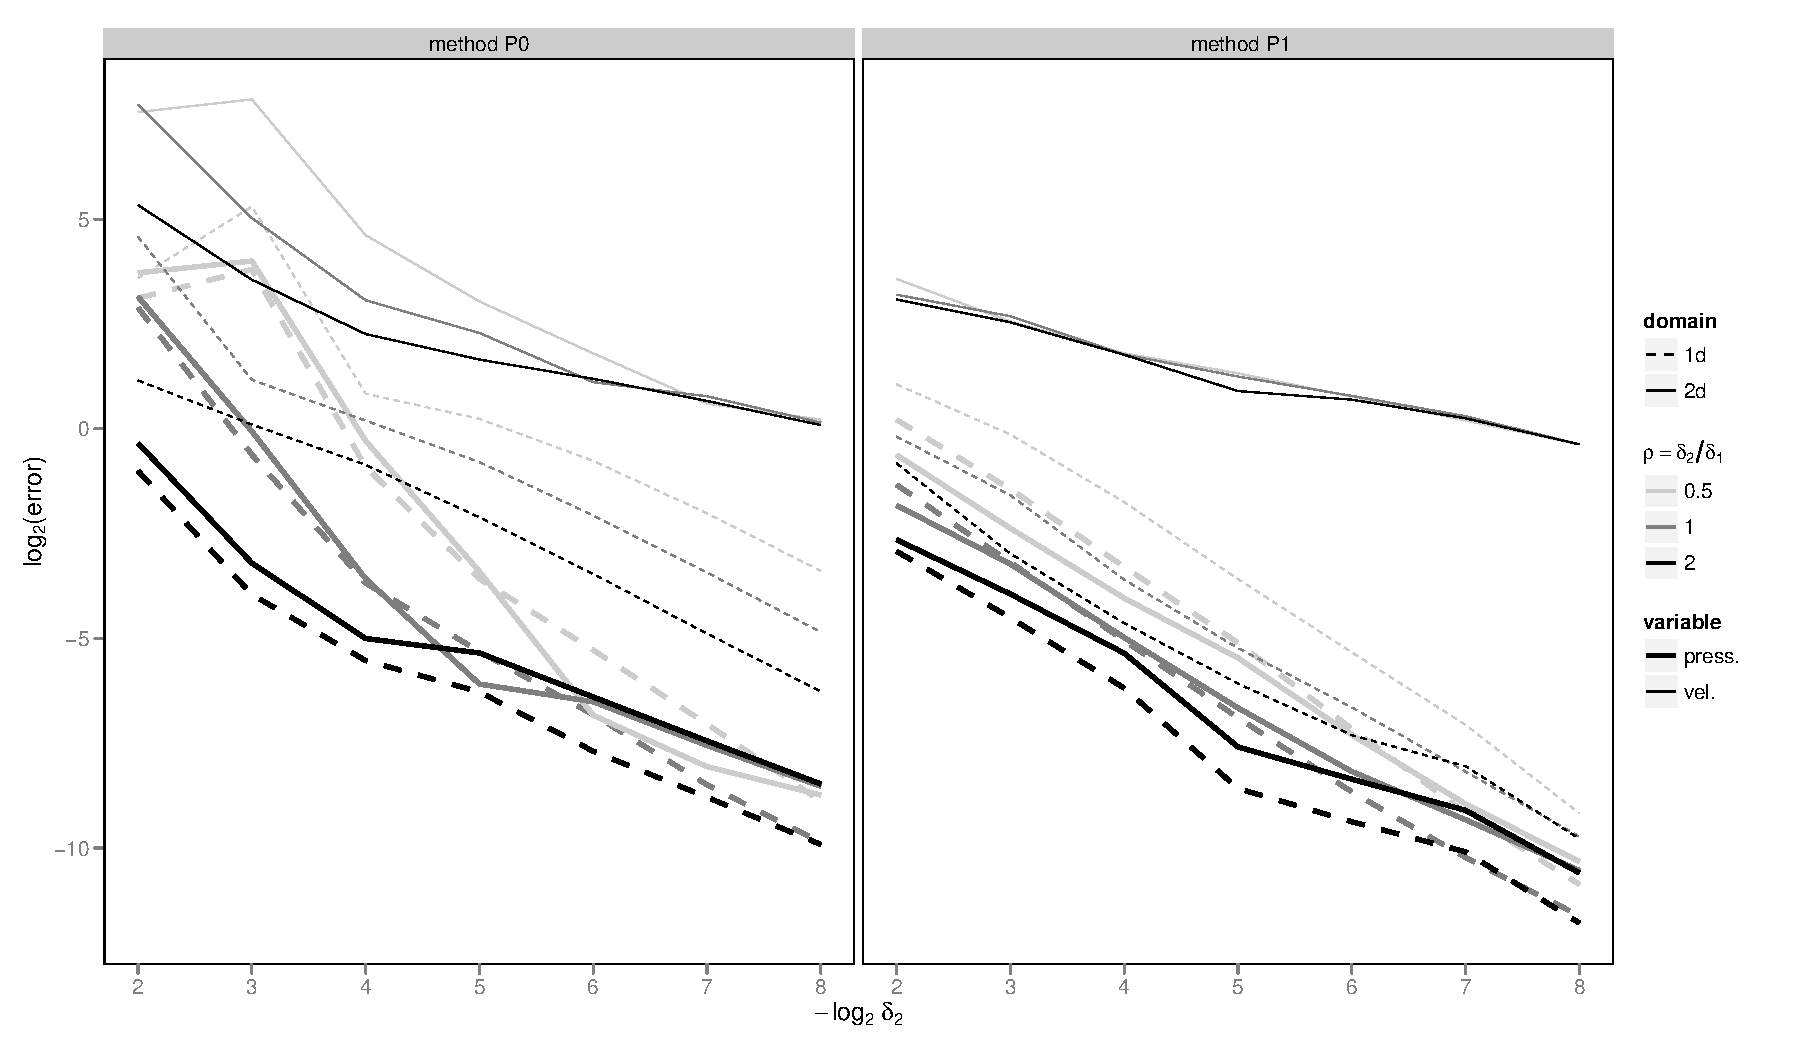
\includegraphics[width=1.00\textwidth, trim=0pt 0pt 23pt 0pt,clip]{./ratio_plot.pdf}
 % ratio_plot.pdf: 720x503 pixel, 72dpi, 25.40x17.74 cm, bb=0 0 720 503
 \caption{Approximative $L^2$-norm of the error for the pressure head and the velocity on both domains and for both methods with $\sigma =100$.}
 \label{fig:ratio}
\end{figure}

Before we proceed to the analysis of the order of convergence, we should discus the role of the parameter $\rho$. 
It is known from the theory of mortar methods that discretization
of the mortar interface (fracture in our case) should not be finer then discretization of the surrounding sub-domains 
(see \cite[Assumption 2.1]{wheeler_efficient_2010}). This condition is not very restrictive in practice, 
however we can demonstrate it in Figure \ref{fig:ratio} that displays errors for the most sensitive case $\sigma=100$.
All black lines, which corresponds to $\rho=2$, have smaller slope at the right hand part of plot that 
corresponds to the fine meshes. 
It means that the order of convergence is slightly deteriorated for large values of $\rho$ in particular for 
the method P0 and for the error of $h_1$. On the other hand, for smaller values of $\rho$, the method P0 exhibits quite large 
errors on coarse meshes. This is caused by bad conditioning of the linear system. In fact for $\rho=0.2$ (not on the plot),
we get completely wrong solution on coarse meshes. The conclusion is that the method P0, unlike the method P1, 
requires $\delta_1$ to be close to $\delta_2$.  

\begin{table}[h]
\caption{Estimated order of convergence of approximated $L^2$-error for the pressure head and the velocity.}
\begin{center}
\begin{tabular}{ r@{\hspace{1em}}  l  l l l @{\hspace{1em}} l  l l l }
 \toprule
 &\multicolumn{4}{ c }{pressure head}
 &\multicolumn{4}{ c }{velocity}\\
 \cmidrule(r){2-5}
 \cmidrule(r){6-9}

 &\multicolumn{2}{ c }{$\rho=0.5$}
 &\multicolumn{2}{ c }{$\rho=1$}
 &\multicolumn{2}{ c }{$\rho=0.5$}
 &\multicolumn{2}{ c }{$\rho=1$}\\
 \cmidrule(r){2-3}
 \cmidrule(r){4-5}
 \cmidrule(r){6-7}
 \cmidrule(r){8-9}
 
           &  1d  & 2d   & 1d   & 2d   &  1d   & 2d   & 1d   & 2d \\
 method P0 &  2.1 & 1.60 & 1.87 & 1.55 &  1.82 & 0.6  & 1.43 & 0.56              \\
 method P1 &  2.1 & 1.68 & 1.87 & 1.55 &  1.82 & 0.6  & 1.60 & 0.56               \\
 compatible mesh
           &  1.9 & 1.9  & 1.9  & 1.9  &  1.9  & 1    & 1.9  & 1 \\
 \bottomrule
\end{tabular}
\label{tab:order}
\end{center}
\end{table}



For estimation of the order of convergence, we have used linear regression and analysis of variance to determine factors
that influence the order of convergence. The results are summarized in Table \ref{tab:order}.  
On the last line, there are also results for the convergence of solution on a compatible mesh.
The values for both methods were very close and different values are reported only when the difference 
was statistically significant. Surprisingly the ratio $\rho$ has stronger impact then the choice of the method. 
Value of the parameter $\sigma$ has no significant influence on the order of convergence. 
On the other hand, the absolute magnitude of all errors save the error $\eta(\vc v_2)$ was two times larger 
for the method P0 then for the method P1.

Comparing to the compatible case, which exhibits almost optimal orders of convergence, the substantial difference is namely 
for $\eta(h_2)$ (about $3/2$ for our method) and for $\eta(\vc v_2)$. Indeed, the order of convergence of the error 
$\eta(\vc v_2)$ should be about $1/2$ since we have constant error  $\eps$ on all elements along 
$\Omega_1$ due to the bad resolution of the jump in the velocity, then 
\[
\eta(\vc v_2) > \sqrt{1/\delta_2 \eps^2 \delta_2^2} = \eps\sqrt{\delta_2}.
\]


The last thing, we want to mention is conditioning of the discrete system. As was already mentioned, the system resulting from the 
discretization is indefinite, but one can apply Schur complements to obtain a reduced positive definite system.
We have used CG solver to solve this system and as the side effect we have obtained approximative eigenvalues,
which allows us to compute estimate of the condition number.
The method P0 and the compatible case has similar condition numbers, but surprisingly 
the method P1 had condition numbers about ten times smaller, which leads to
the less than half number of iterations. This property is unaffected by $\sigma$, $\rho$ or $\delta_2$.

\section{Conculsions}
We have presented two new methods for the mixed-hybrid discretization of couplings between dimensions. Both methods 
were tested on a simple 2d-1d problem that provides an analytical solution. The experimentally determined orders of convergence 
are almost same for both methods, but the absolute errors are smaller for the method P1. 
This method also results into  linear systems with better condition numbers and is more robust.
The main drawback of both methods is worse resolution of the velocity near the fractures. 
 




\bibliographystyle{plain}
\bibliography{nonmatching_grids}

\end{document}














